\section{Konzepte}
\subsection{Mechanik}
\begin{frame}
	\frametitle{Konzepte}
	\framesubtitle{\textit{Titanium Ores}}
	\vspace{-1em}
	\begin{figure}		
		\begin{tikzpicture}[scale=1, transform shape]
		\def\height{4.5cm}
		\node[anchor=south west,inner sep=0] (image) at (0,0) {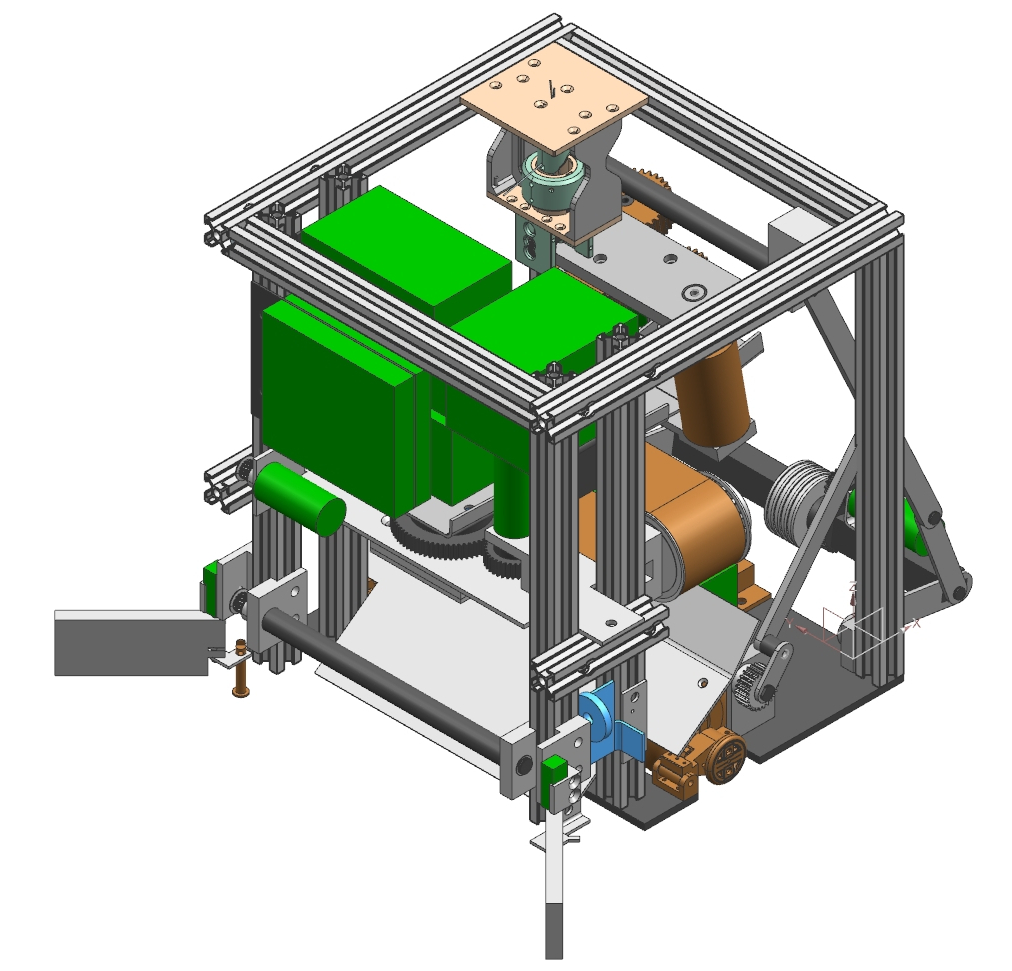
\includegraphics[height=5.5cm] {../images/mechKonzept/Roboter_grossPres.jpg}};
		
		\begin{scope}[xshift=6cm]
		\node[anchor=south west,inner sep=0] (rimage) at (0,1) {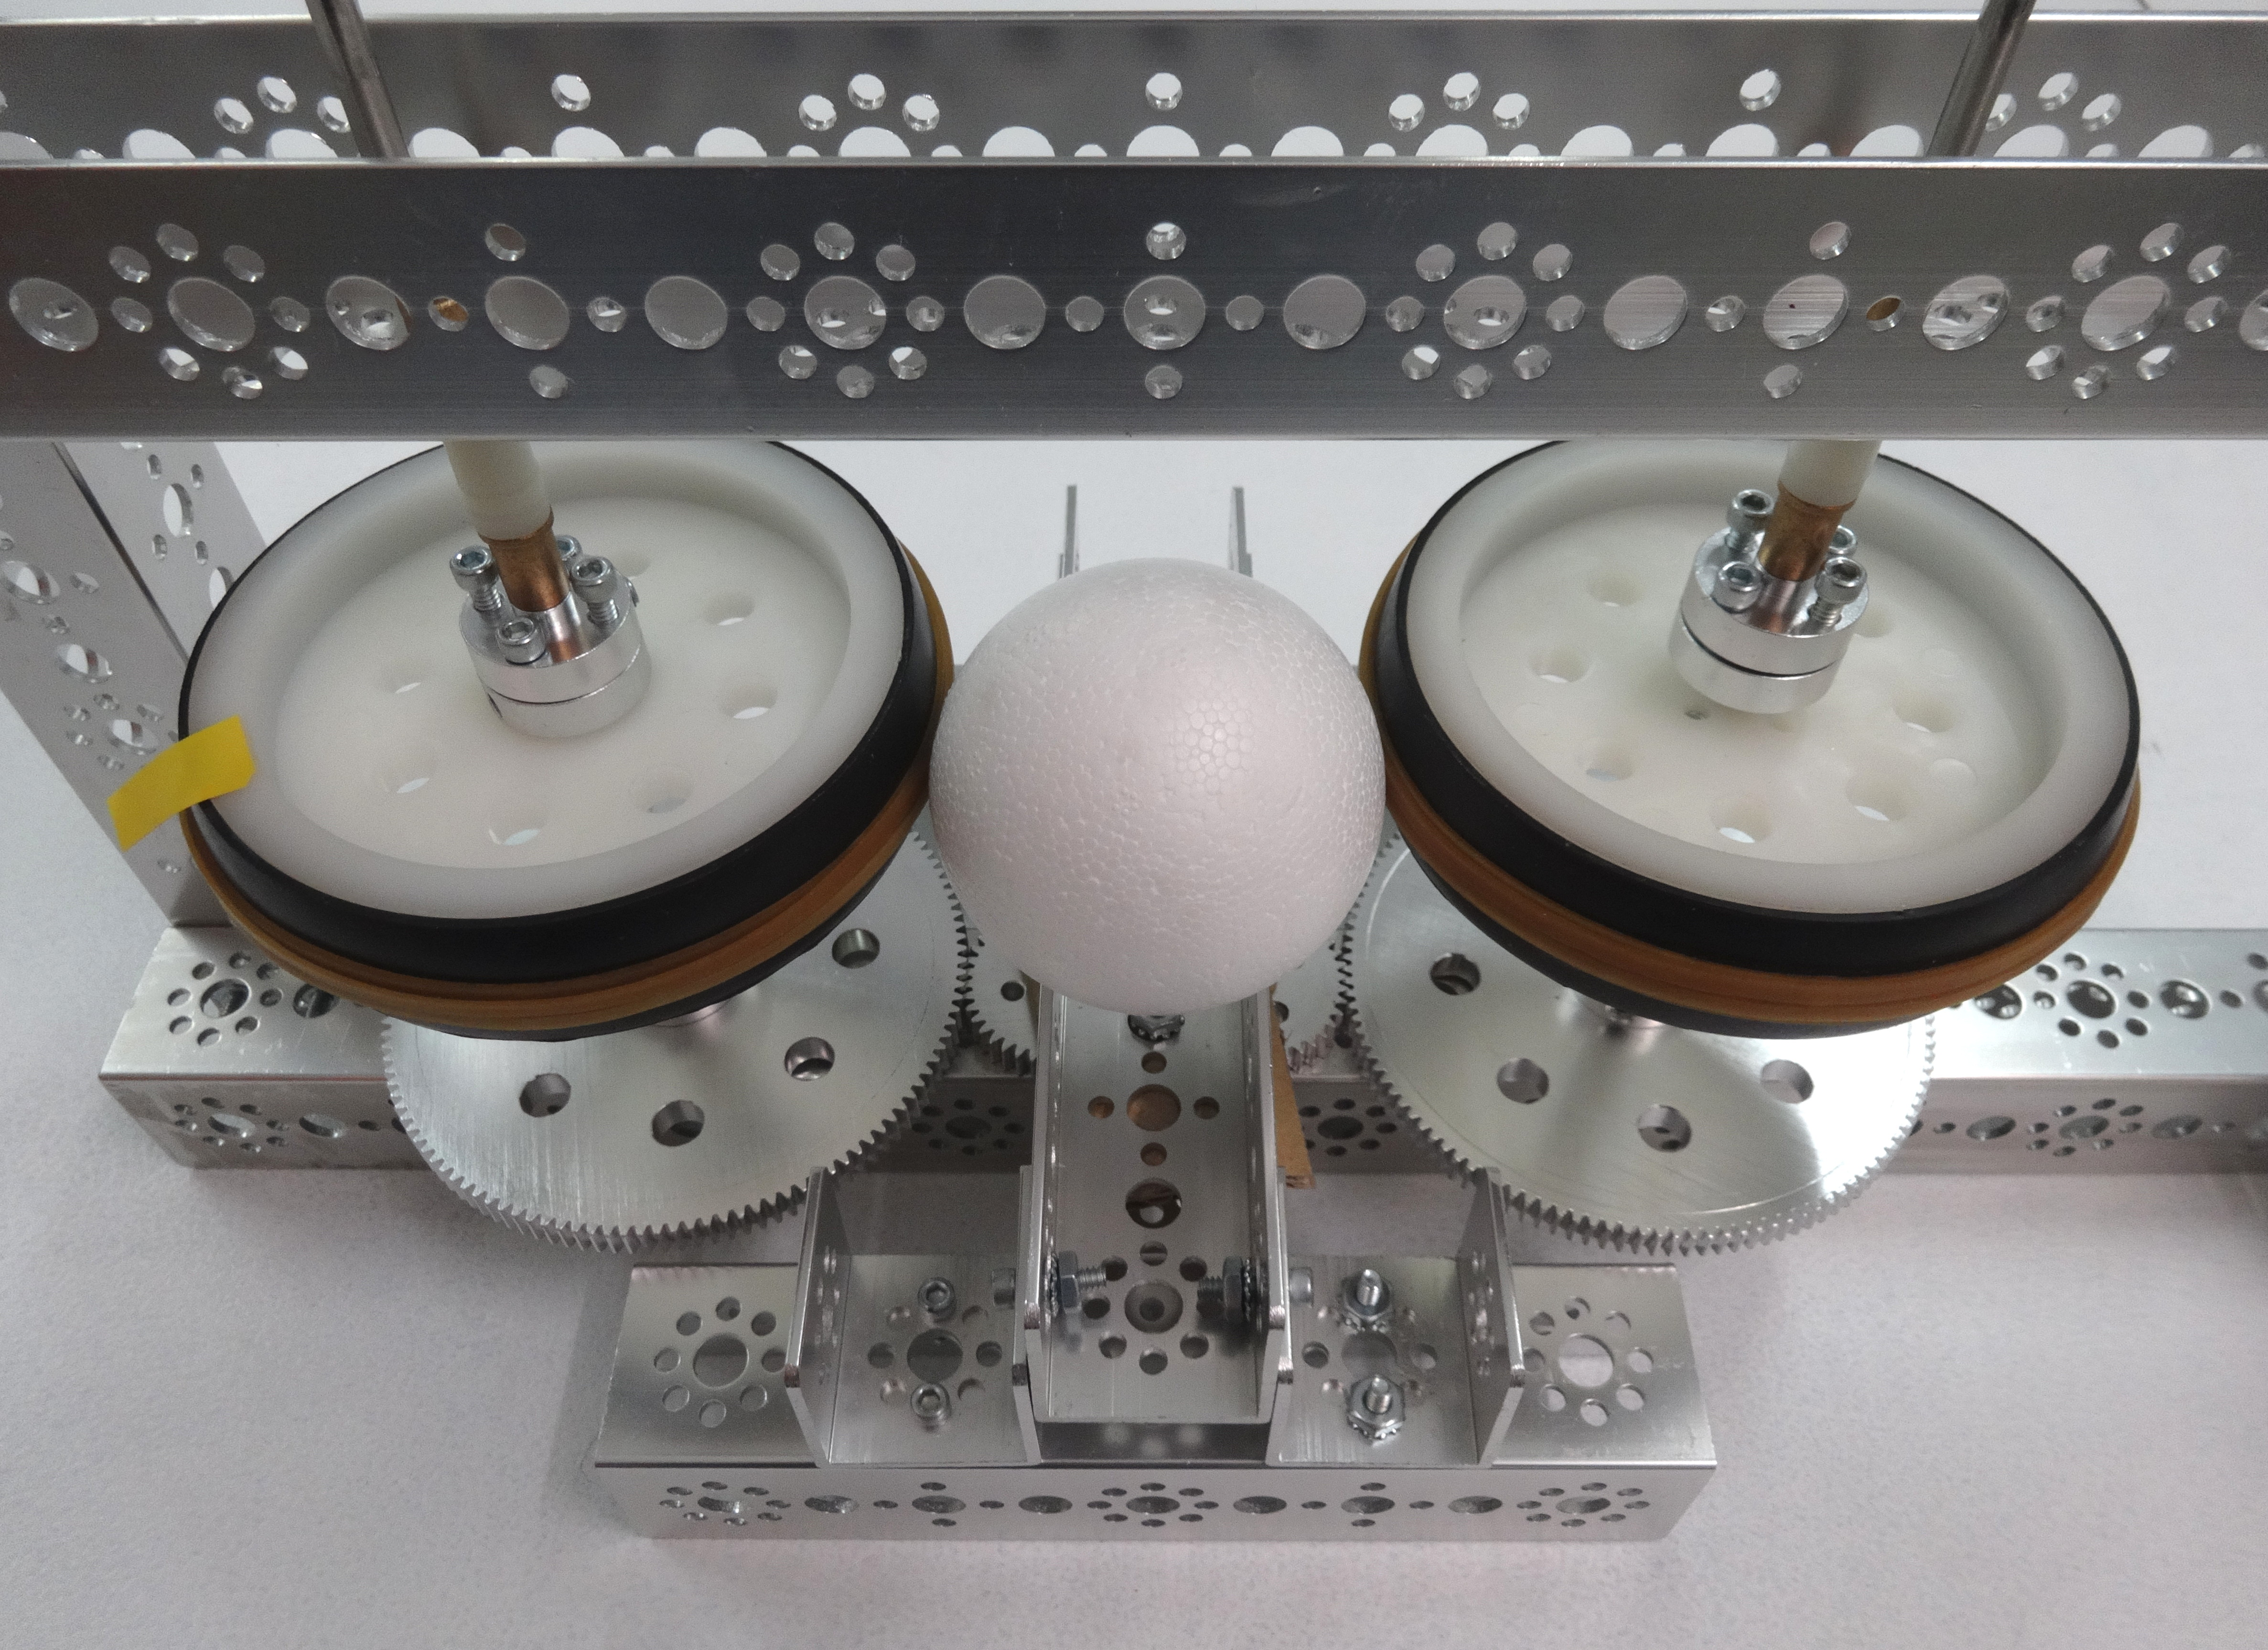
\includegraphics[height=3.5cm] {../images/mechKonzept/Ballschussanlage2.JPG}};
		
		\end{scope}
		\end{tikzpicture}	
		
		\vspace{1em}
		CAD-Modell grosser Roboter und Versuchsaufbau Ballschussmaschine
	\end{figure}

\end{frame}    

\begin{frame}
	\frametitle{Konzepte}
	\framesubtitle{\textit{Lunar Modules}}
	
	\begin{figure}
		\begin{tikzpicture}[scale=1, transform shape]
		\def\height{5cm}
		\node[anchor=south west,inner sep=0] (image) at (0,1) {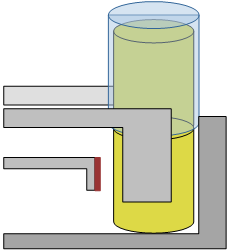
\includegraphics[height=3cm] {../images/mechKonzept/SchrankenPres.png}};
			
		\begin{scope}[xshift=4cm]
		\node[anchor=south west,inner sep=0] (rimage) at (0,0) {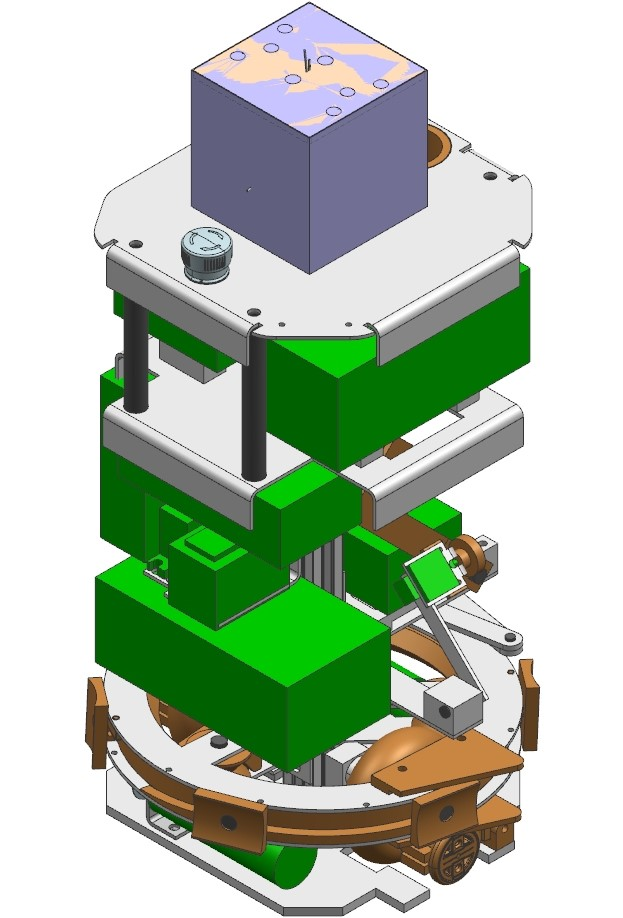
\includegraphics[height=\height] {../images/mechKonzept/Roboter_kleinPres.jpg}};
		
		\end{scope}
		\end{tikzpicture}	
		\vspace{1em}
		
		Prinzip Modulaufnahme und CAD-Modell kleiner Roboter
	\end{figure}

	  
\end{frame}

\subsection{Gesamtsystem}
\begin{frame}
	\frametitle{Elektronikmodule}
	
	\vspace{-1em}	
	\begin{figure}
		\begin{tikzpicture}[scale=0.6, every node/.style={scale=0.5}]
		% box for Robot
		\draw [color=cBlue, line width=0.6mm, rounded corners=2pt] (-2,15) node[below right]{\Large Roboter} rectangle (16,4.5);
		
		% box for Mainboard
		\draw [color=cGreen, line width = 0.4mm, rounded corners = 2pt] (4,12) rectangle (7, 10) node[pos=0.5, color=black]{\Large Mainboard};
		
		% box für Drive Controller
		\draw [color=cGreen, line width = 0.4mm, rounded corners = 2pt] (3,8) rectangle (6,6) node[pos=0.5, text width = 2.5cm, align=center, color=black] {\Large Drive \\ Controller \\ (DC)};
		
		% box für Oponent Detection
		\draw [color=cGreen, line width = 0.4mm, rounded corners = 2pt] (7,8) rectangle (10,6) node[pos=0.5, text width = 2.5cm, align=center, color=black] {\Large Oponent \\ Detection \\ (OD)};
		
		% draw CAN bus
		\draw [line width = 0.8mm] (5.5,10) -- (5.5,9) (2.5,9) node[above right] {CAN Bus} -- (11.5,9) (4.5,9) -- (4.5,8) (8.5,9) -- (8.5,8);
		
		%draw Display
		\draw [line width = 0.4mm, color = cRed, rounded corners = 2pt] (9,14.5) rectangle (12,13.5) node[pos=0.5, color=black] {\Large Display};
		\draw [line width = 0.4mm, rounded corners = 2pt] (6,12) -- (6,14) node[above right]{SPI} -- (9,14);
		
		%draw Bluetooth
		\draw [line width = 0.4mm, color = cRed, rounded corners = 2pt] (9,13) rectangle (12,12) node[pos=0.5, color=black] {\Large Bluetooth};
		\draw [line width = 0.4mm, rounded corners = 2pt] (6.5,12) -- (6.5,12.5) node[above right]{UART} -- (9,12.5);
		
		%draw Datenlogger
		\draw [line width = 0.4mm, color = cRed, rounded corners = 2pt] (9,11.5) rectangle (12,10.5) node[pos=0.5, color=black] {\Large Datenlogger};
		\draw [line width = 0.4mm, rounded corners = 2pt] (7,11) node[above right]{UART} -- (9,11);
		
		%draw Powerboard
		\draw [line width = 0.4mm, color=cGreen, rounded corners = 2pt] (2,14.5) rectangle (5,13) node[pos=0.5, color=black] {\Large Powerboard};
		\draw [line width = 0.4mm, rounded corners = 2pt] (2.5,13) -- (2.5,11) node[above right] {Direkt} -- (4,11);
		
		%draw LED ring
		\draw [line width = 0.4mm, color = cRed, rounded corners = 2pt] (12.4,7.5) rectangle (15.5,8.5) node[pos=0.5, color=black] {\Large LED Ring};
		\draw [line width = 0.4mm, rounded corners = 2pt] (10,7.5) -- (10.5,7.5) -- (10.5,8) node[above right]{SPI} -- (12.4,8);
		
		%draw OD motoren und sensoren
		\draw [line width = 0.4mm, color = cRed, rounded corners = 2pt] (12.4,6) rectangle (15.5,7) node[pos=0.5, color=black] {\Large Motor, Sensoren};
		\draw [line width = 0.4mm, rounded corners = 2pt] (10,6.5) node[above right]{Direkt} -- (12.4,6.5);
		
		%draw 9 achsen sensor
		\draw [line width = 0.4mm, color = cRed, rounded corners = 2pt] (-1.5,8) rectangle (1.6,9) node[pos=0.5, color=black] {\Large 9-Achsen Sensor};
		\draw [line width = 0.4mm, rounded corners = 2pt](1.6,8.5) node[below right, xshift=0.5cm]{I$^2$C}-- (4,8.5) -- (4,8);
		
		%Schleppräder
		\draw [line width = 0.4mm, color = cRed, rounded corners = 2pt] (-1.5,7.5) rectangle (1.6,6.5) node[pos=0.5, color=black] {\Large Schleppräder};
		\draw [line width = 0.4mm, rounded corners = 2pt] (1.6,7) -- (3,7) node[below left]{SPI};
		
		%Motoren
		\draw [line width = 0.4mm, color = cRed, rounded corners = 2pt] (-1.5,6) rectangle (1.6,5) node[pos=0.5, color=black] {\Large Motoren};
		\draw [line width = 0.4mm, rounded corners = 2pt] (1.6,5.5) -- (4,5.5) node[below left]{PWM} -- (4,6);
		
		\end{tikzpicture}
	\end{figure}

\end{frame}

\begin{frame}
	\frametitle{Sensoren und Aktoren}
	
	\begin{itemize}
		\item Diverse Motoren, Servoantriebe und Sensoren nötig
		\item Wenn möglich Servos vorgesehen %Intelligente Servos, normale Servos, DC-Motoren für grössere Drehbereiche und wo Kraft nötig ist
		\item Sensoren: nur Farbsensor zur Erkennung Modulfarbe ausgewählt
	\end{itemize}   

	\begin{figure}
		\captionsetup[subfigure]{font=scriptsize,labelfont=scriptsize}
		\begin{subfigure}{0.2\textwidth}
			\centering
			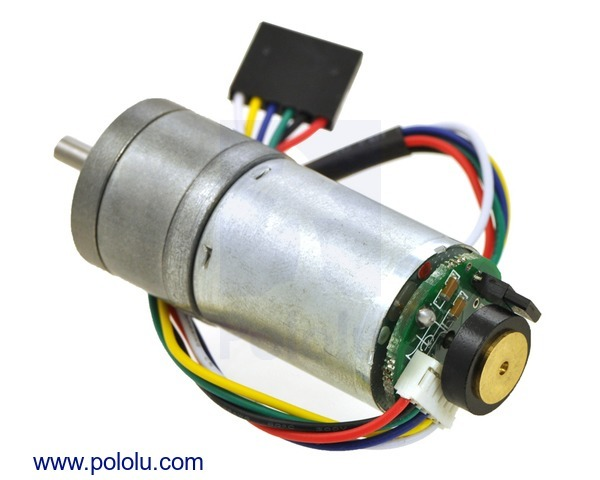
\includegraphics[height=2cm] {../images/presentation/DCMotor.jpg}
			\subcaption*{Quelle: popolu.com}
		\end{subfigure}
		\hspace{1em}
		\begin{subfigure}{0.2\textwidth}
			\centering
			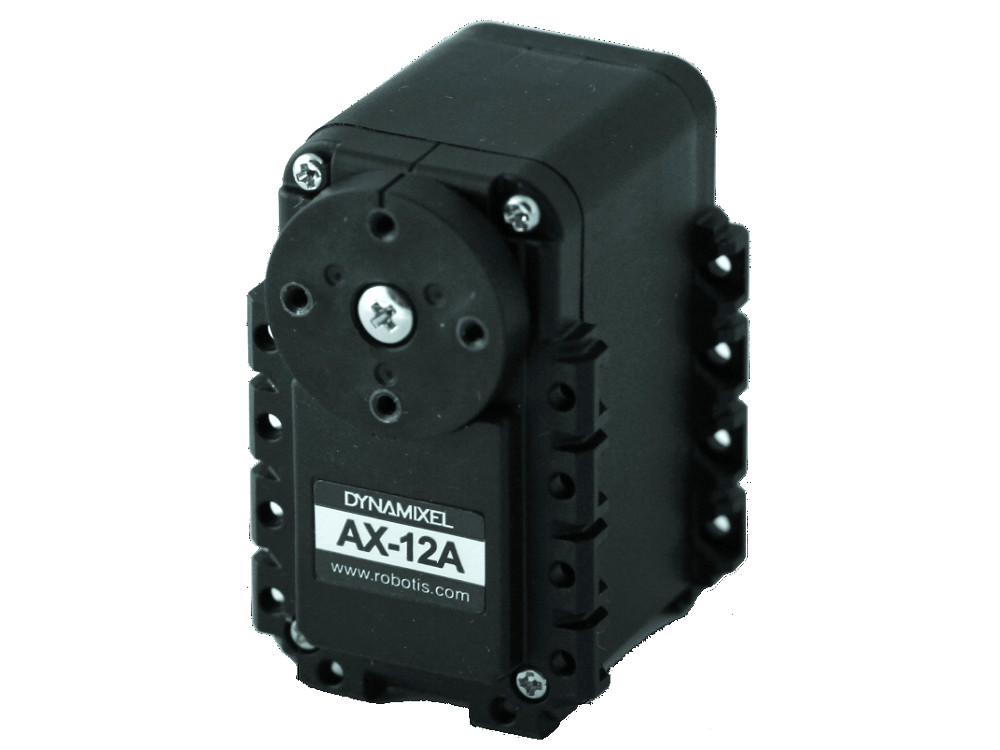
\includegraphics[height=2cm] {../images/presentation/IntServo.jpg}
			\subcaption*{Quelle: diigiit.com}
		\end{subfigure}
		\hspace{1em}
		\begin{subfigure}{0.2\textwidth}
			\centering
			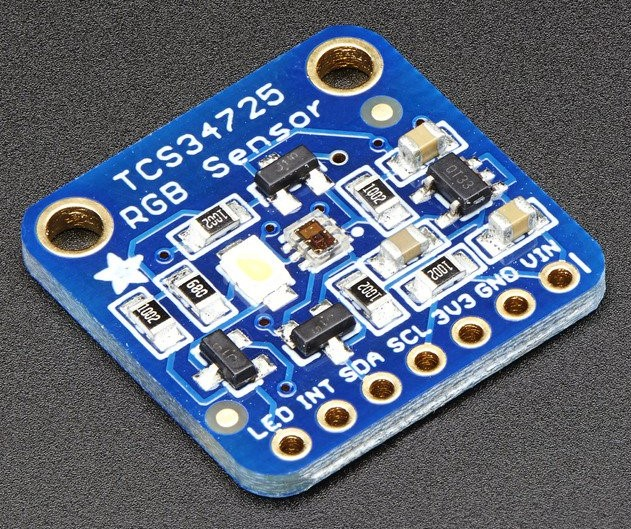
\includegraphics[height=2cm] {../images/presentation/RGB.jpg}
			\subcaption*{Quelle: adafruit.com}
		\end{subfigure}
		\hspace{1em}
	\end{figure}
	
	%Quelle: https://cdn-shop.adafruit.com/970x728/1334-04.jpg
	%Quelle: https://a.pololu-files.com/picture/0J3799.600x480.jpg?03a71976857bd4e6d447a7cd8817f31c
	%Quelle: http://www.eu.diigiit.com/dynamixel-ax-12a
\end{frame}